\renewcommand*{\mypath}{superapp}%
\graphicspath{ {\mypath/images/} }

\doctitle{Lorenzo Affetti}{lorenzo.affetti@polimi.it}

\section{Introduzione}
Lo scopo dell'applicazione SuperApp è quello di mettere in atto una collaborazione tra quattro giocatori attraverso diverse modalità di gioco.
Ogni giocatore della squadra gioca su un tablet diverso, uno \textit{slave}. Il gioco necessita di un ulteriore tablet, il \textit{master}, che non verrà utilizzato da nessun giocatore, ma che fornirà informazioni di massima sulla partita in corso e scandirà le partite e le manche di gioco.

I dispositivi comunicano per mezzo di una connessione \textit{Bluetooth}. Un disegno di massima delle posizioni dei tablet è fornito in figura \ref{fig:tablet5}.

\begin{figure}[h!]
\centering{
\includegraphics[width=\textwidth]{tablets.png}}
\caption{I cinque tablet}
\label{fig:tablet5}
\end{figure}

L'applicazione comprende tre diversi giochi:

\begin{itemize}
\item \textit{Trova l'Intruso}: I giocatori devono, appunto, trovare l'intruso. Ad un certo numero di risposte esatte consecutive (configurabile) la logica di gioco si inverte (vengono dati feedback sonori e visivi) e il gioco diventa, quindi, trova il \textit{non} intruso. Questo gioco può essere lanciato in quattro diverse modalità: trova l'intruso per colore, \textit{ancora-colore} (come la modalità per colore, con la differenza che le immagini vengono mostrate in bianco e nero all'inversione di gioco), direzione e forma. 
\item \textit{Ordina dal Più Piccolo al Più Grande}: I giocatori devono ordinare quattro oggetti dal più piccolo al più grande o viceversa.
\item \textit{Costruisci la Torre}: I giocatori devono completare una torre composta da quattro oggetti giocando a turno.
\end{itemize}

In ognuno dei tre giochi l'applicazione sottopone agli utenti delle immagini che si muovono con velocità variabile su dei nastri trasportatori.

Ogni \textit{partita} è composta da un numero di \textit{manche} (o anche \textit{stage}) configurabile. Il completamento di tutte le manche porta alla vittoria del gruppo. I punteggi sono sempre cumulativi dell'intera squadra.

\section{Struttura Generale}
% struttura generale delle classi (3 modalità di gioco -> ereditarietà)
% TODO class diagram di altissimo livello

% la comunicazione ad eventi:
% - Otto
% - le categorie di eventi
% - i vari pattern di comunicazione
% TODO diagramma di interazione back <-> front (con tanto di eventi)

\begin{figure}[h!]
\centering{
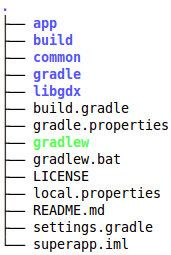
\includegraphics{tree_root.png}}
\caption{La struttura del progetto (profondità 1)}
\label{fig:tree_root}
\end{figure}

Il codice sorgente dell'applicazione è suddiviso in tre moduli (figura \ref{fig:tree_root}). Il modulo \code{app} contiene il backend comprensivo di logica di comunicazione e il frontend dell'applicazione. Il modulo \code{libgdx} contiene le parti più interattive dell'applicazione e cioè quelle dei nastri trasportatori. Infine, il modulo \code{common} contiene moduli privi di dipendenze dal framework di Android e usati in ambedue i precedenti moduli.

Come già accennato, SuperApp è divisa in tre diversi giochi di cui il primo è disponibile in quattro modalità diverse (in realtà, anche il secondo, tuttavia la logica di gioco rimane invariata tra di esse, ciò che varia è solo l'ordinamento delle quattro immagini iniziali). Per questo motivo, quasi ogni classe costituente il nucleo della logica di gioco (si veda \ref{subsec:logic}) e diversi \textit{fragment} (si veda \ref{subsec:activities}) segue il particolare schema di ereditarietà illustrato in figura \ref{fig:hierarchy}, a parte sporadiche eccezioni che, però, sono facilmente comprensibili a una prima lettura del codice (per esempio, abbiamo \code{Slave1Color} e \code{Slave1ColorAgain}, ma solo un \code{MasterColor} poiché il ruolo del \textit{master} nelle due modalità non cambia).

\begin{figure}[h!]
\centering{
\includegraphics[width=\textwidth]{hierarchy.png}}
\caption{Lo schema di ereditarietà generale}
\label{fig:hierarchy}
\end{figure}

\section{Backend}

\subsection{Il TenBus}
% spiegare funzionamento TenBus:
% - BTThread
% - Peer
Prima di spiegare il funzionamento di qualsiasi altro componente di SuperApp è necessario introdurre il \code{TenBus}, parte del package \code{it.playfellas.superapp.network}. Questa classe è quella che permette a tutte le componenti del sistema di comunicare tra di loro sia in remoto che in locale. Il \code{TenBus} è un \textit{wrapper} attorno al famoso \textit{bus} ad eventi \textbf{Otto} (\url{http://square.github.io/otto/}).

Dopo aver ottenuto un'istanza del \code{TenBus} tramite il metodo statico \code{get}, un oggetto può \code{post}are \code{NetEvent} oppure \code{InternalEvent}. I primi verranno inviati in remoto sul canale \textit{Bluetooth}, i secondi verranno propagati in locale usando l'originale Otto. Gli eventi sono di molteplici tipi e le loro classi sono contenute nel package \code{it.playfellas.superapp.events}. La generazione di questi ultimi e accentrata nella \code{EventFactory}.

Se un oggetto volesse ricevere degli eventi, dovrà semplicemente invocare il metodo \code{register} passando un qualsiasi oggetto (anche \code{this}) che abbia registrato dei metodi tramite l'annotazione \code{@Subscribe}. I methodi annotati devono accettare in ingresso un oggetto di tipo uguale all'evento interessato e ritornare un valore \code{void}.

Il \code{TenBus} offre anche i metodi \code{attach} e \code{detach} per permettere lo scambio di eventi in remoto. Per il funzionamento dettagliato della connessione \textit{Bluetooth} (inizializzazione, chiusura) si veda il codice.

Le classi \code{BTThread} e \code{Peer} (e quelle che le estendono) sono volutamente invisibili all'esterno del package \code{network}, l'unico punto d'accesso alla rete per un oggetto esterno è il \code{TenBus}.

\subsection{La Logica di Gioco}
\label{subsec:logic}
% cos'è un Controller?
% e un TileDispenser?
% la GameHistory?

% TODO sequence: cosa succede onClick?

\section{Frontend}

\subsection{Le Activity e i Fragment}
\label{subsec:activities}
% citare ButterKnife
% TODO sequence di interazione

\subsection{I Nastri}
% libgdx e bla bla bla
